\documentclass[final]{siamltex}
\usepackage{geometry}   % See geometry.pdf to learn the layout
                        % options.  There are lots.
\usepackage{graphicx}
\usepackage{epstopdf}
\usepackage{color,amsmath,latexsym,amsfonts,amssymb}

\DeclareGraphicsRule{.tif}{png}{.png}{`convert #1 `dirname #1`/`basename #1 .tif`.png}

%-----Extra Formatting Options
\textheight 9.0truein
\textwidth 6.5truein
\addtolength{\topmargin}{-0.25in}
\addtolength{\evensidemargin}{-0.5in}
\setlength{\parindent}{0em}
\setlength{\parskip}{2ex}

%----My Definitions---
\renewcommand{\(}{\left(}
\renewcommand{\)}{\right)}
\newcommand{\dt}{\Delta t}
\newcommand{\R}{\mathrm R}
\newcommand{\N}{\mathrm N}
\newcommand{\alfven}{Alfv\'{e}n }
\newcommand{\sundials}{\normalfont\scshape Sundials}
\newcommand{\fninety}{\normalfont\scshape Fortran90}
\newcommand{\kinsol}{\normalfont\scshape KINSol}
\newcommand{\cvode}{\normalfont\scshape Cvode}
\newcommand{\openad}{\normalfont\scshape OpenAD}
\newcommand{\hypre}{\normalfont\scshape Hypre}
\newcommand{\superlu}{\normalfont\scshape SuperLU}
\newcommand{\petsc}{\normalfont\scshape PETSc}
\newcommand{\tao}{\normalfont\scshape TAO}
\newcommand{\trilinos}{\normalfont\scshape Trilinos}
\newcommand{\bbeta}{{\bf \beta}}
\newcommand{\bU}{{\bf U}}
\newcommand{\tU}{{\tilde{\bf U}}}
\newcommand{\bV}{{\bf V}}
\newcommand{\bW}{{\bf W}}
\newcommand{\bF}{{\bf F}}
\newcommand{\bG}{{\bf G}}
\newcommand{\bH}{{\bf H}}
\newcommand{\bS}{{\bf S}}
\newcommand{\pt}{\tilde{p}}
\newcommand{\tbF}{\tilde{\bF}}
\newcommand{\tbG}{\tilde{\bG}}
\newcommand{\tbH}{\tilde{\bH}}
\newcommand{\mI}{{\mathcal I}}
\newcommand{\mJ}{{\mathcal J}}
\newcommand{\mR}{{\mathcal R}}
\newcommand{\bu}{{\bf u}}
\newcommand{\bB}{{\bf B}}


%----Head Matter-------------------------------------------
\title{Parallel Solvers for Linear Systems On Structured Grids} 
\author{Samuel H. White \& Daniel R.~Reynolds\\
  (Two Semester Project)
} 
%\email{shwhite@smu.edu, reynolds@smu.edu}
%\date{August 15, 2011}

%----Begin Document----------------------------------------
\begin{document}

\maketitle

\pagestyle{myheadings}
\thispagestyle{plain}
\mark{S..H.~White \& D.R.~Reynolds -- Parallel Solvers for Structured Grids}


\section{Introduction}
\label{sec:intro}

In recent years, numerical simulation has rapidly become the third
pillar of scientific insight, joining experiment and theory as the
primary tools through which we explore the world around and within us.
At the core of numerical simulations in physics, engineering and 
biology reside mathematical models posed as systems of partial
differential equations (PDEs).  In mathematically approximating
solutions to these continuum-level models, scientists traditionally
develop a hierarchy of discretizations, where each level of this
hierarchy provides a more thorough and highly-resolved solution for
the underlying continuum PDE model.  Moreover, solution methods for
these discrete models typically require solving systems of
linear equations, where the size of these linear systems is
proportional to the fidelity of the discrete model under study.  In
modern scientific applications, these linear systems can range in size
from problems with millions of equations and unknowns for typical
desktop computers, to problems with trillions of equations and
unknowns for cutting-edge supercomputers.

In previous work, we have applied novel solution algorithms for
almost-supercomputer-sized models of magnetically confined fusion
plasmas \cite{ReynoldsSamtaneyWoodward2006,ReynoldsSamtaneyWoodward2010}.
While these methods are somewhat complex, their ultimate utility
resides in the speed, accuracy and parallel scalability
of a single computational routine, or kernel.  In
the proposed project, we wish to develop and implement a novel
algorithm for this kernel, that will extend both its accuracy and
scalability, with potential and wide-ranging applications in
computational science and applied mathematics.



\section{Problem Description}
\label{sec:problem}

We consider solvers for PDE systems posed on structured grids, as
shown in Figure \ref{fig:plots}a.
\begin{figure}[t]
\begin{minipage}[l]{0.3 \textwidth}
\caption{Clockwise from top left: 
  (a) Three-dimensional problem domain, where each box represents a
  set of model discretization data; (b) decomposition of the
  computational domain among parallel processors, each group of boxes
  corresponds to a distinct processor; (d) nonzero
  structure of tridiagonal matrix; (c) nonzero structure of
  heptadiagonal matrix (zoomed out to see all 7 bands, with space
  separating each).} 
\label{fig:plots}
\vspace{2.4cm}

\end{minipage}
\hspace{0.2cm}
\begin{minipage}[r]{0.6 \textwidth}
\centering
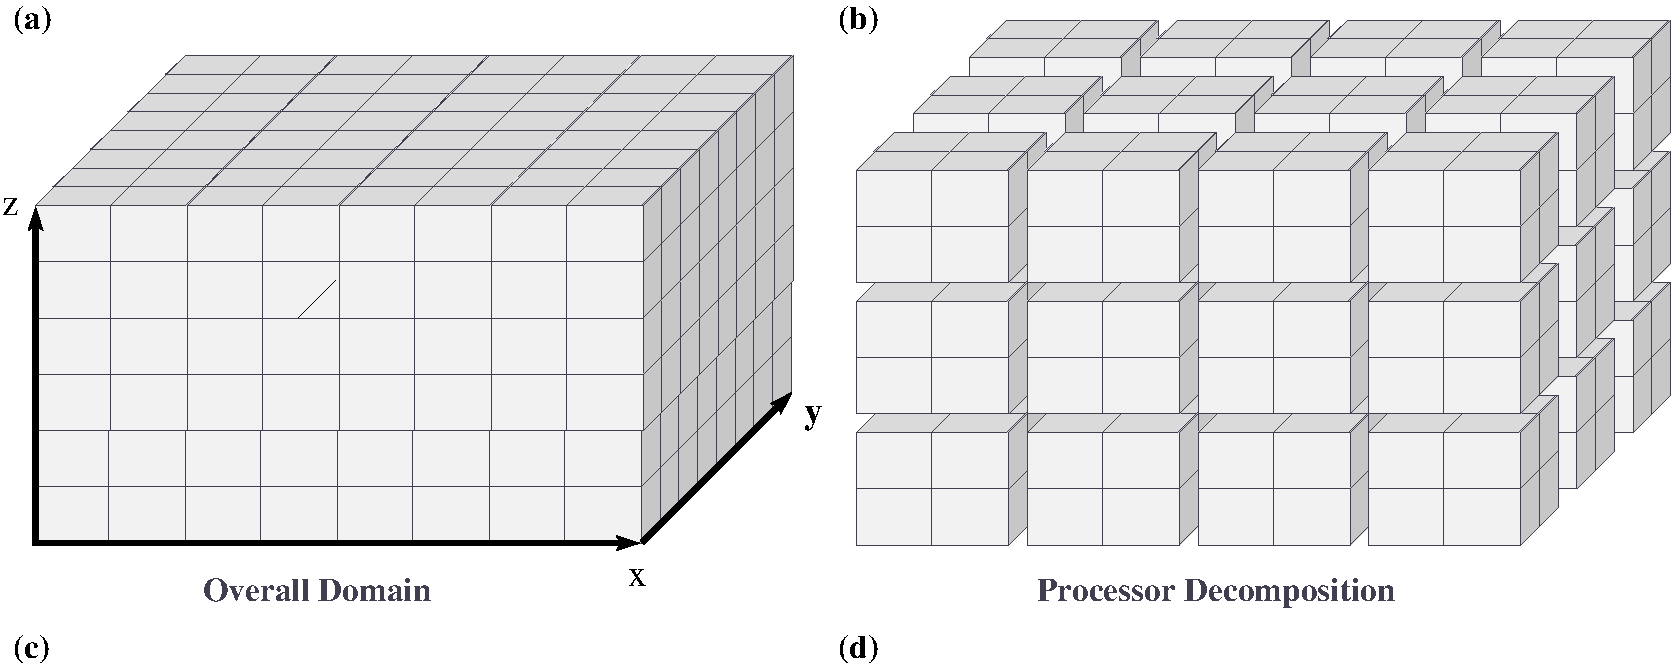
\includegraphics[scale=0.35]{dom_decomp} 
%\vspace{0.25cm}

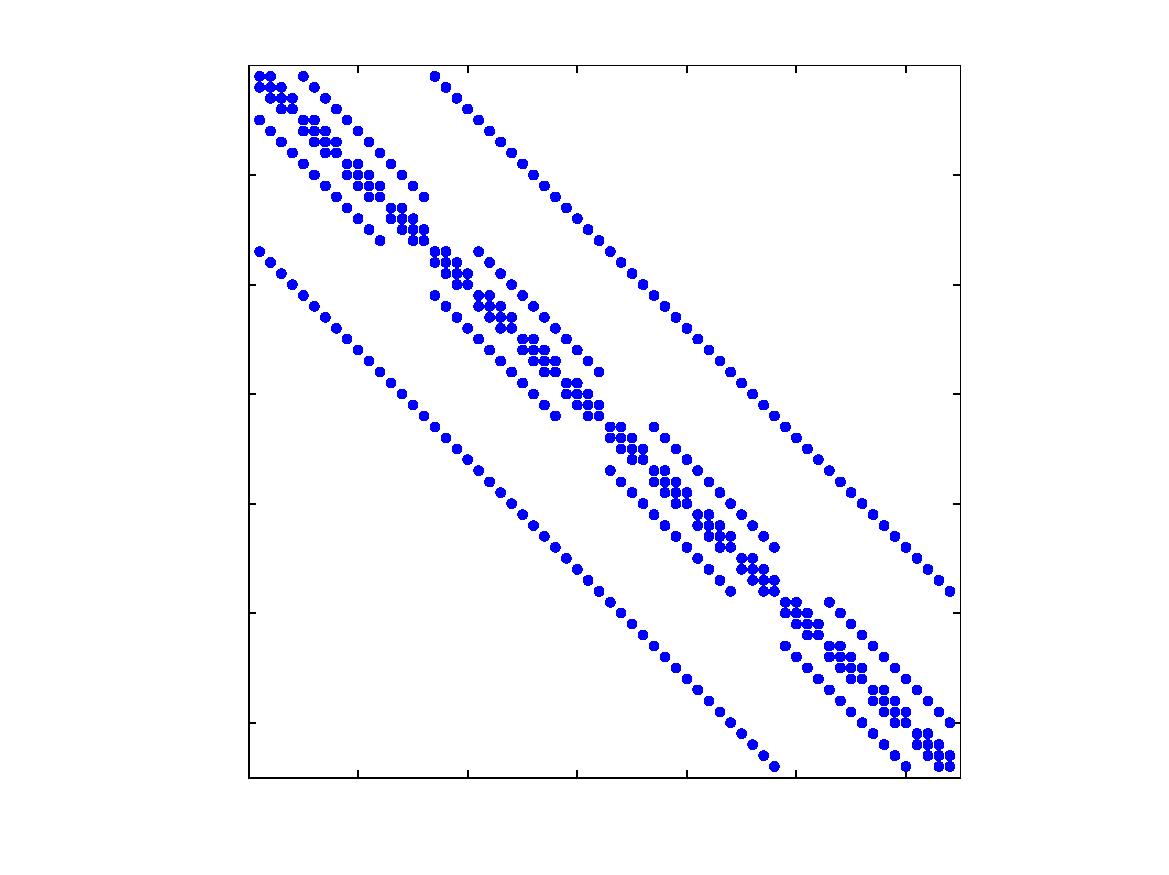
\includegraphics[scale=0.34]{heptadiag}
\hspace{0.5cm}
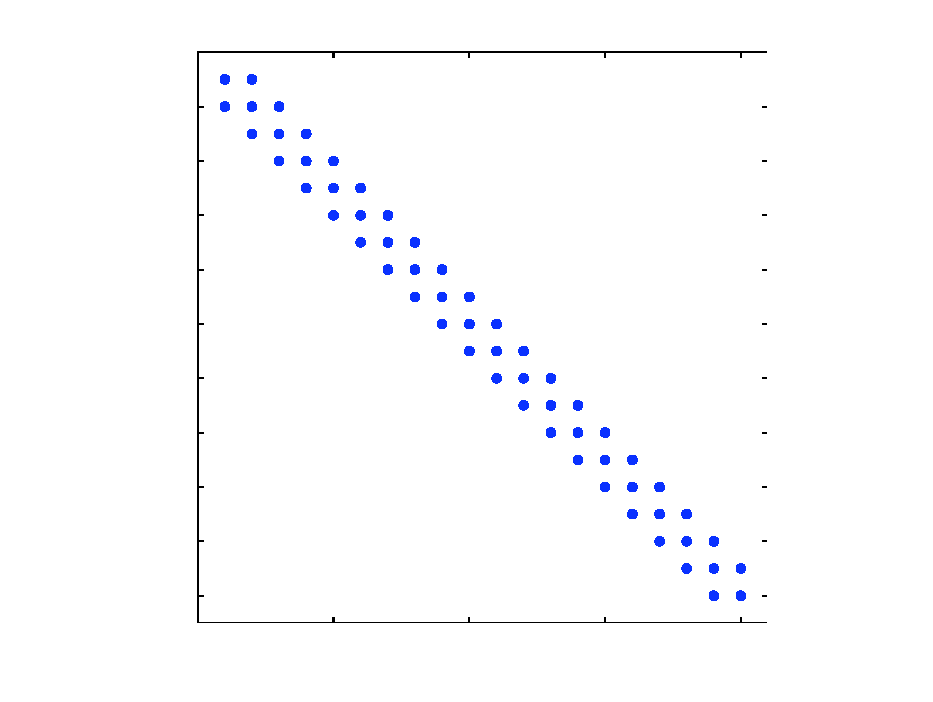
\includegraphics[scale=0.43]{tridiag}
\end{minipage}
\end{figure}
Each small cube in the figure represents a set of discretization data.  As
the model resolution increases, the size of this data grows, and
eventually cannot reside on a single computer, so the domain must be 
decomposed among different nodes of a parallel computer, as
illustrated in Figure \ref{fig:plots}b. 

Over this domain, we must solve linear systems of equations,
$A\vec{x}=\vec{b}$, where $A$ is a very large, square, nonsingular
matrix, and $\vec{x}$ and $\vec{b}$ are appropriately-sized solution
and data vectors, respectively.  For a wide class of PDE models posed
on 3D structured grids, $A$ has a special heptadiagonal structure, as
shown in Figure \ref{fig:plots}c.  When $A$ is very large, basic
solution algorithms become intractable, and approximate solvers must be
used to find $\vec{x}$. 



\section{Solution Approach}
\label{sec:solvers}

The unique heptadiagonal structure of $A$ results from the fact that
it is comprised as the sum of matrices that each act along a single
coordinate direction,
\begin{equation}
\label{eq:A}
   A \ = \ I + A_x + P A_y P^T + Q A_z Q^T,
\end{equation}
where $P$, $Q$, $P^T$ and $Q^T$ are permutation matrices that reorder
the indices in a linear system, and where each of the matrices
$A_x$, $A_y$ and $A_z$ are tridiagonal, as shown in Figure
\ref{fig:plots}d.  The linear system $A\vec{x}=\vec{b}$ may then be
approximately solved using the splitting
\[
   \vec{x} \ = \ A^{-1}\vec{b} 
   \ \approx \ Q(I + A_z)^{-1}Q^TP(I + A_y)^{-1}P^T(I + A_x)^{-1}b.
\]
On a single computer, each of the tridiagonal solvers $(I+A_*)^{-1}$
may be performed using the highly-efficient {\em Thomas algorithm}
\cite{Conte1972}. In our previous work for fusion plasma models, we
created a parallelized version of this algorithm to achieve a highly
scalable and efficient code that effectively used over 1000 parallel processors 
\cite{ReynoldsSamtaneyWoodward2010}.  However, our basic
implementation of that algorithm suffers from an accumulation of
computer roundoff error as the problem grows, effectively limiting its 
eventual utility to the $\sim\!\!1000$ processor range, which although
is respectable, is a far cry from modern supercomputers with over
100,000 processors.  However, thanks to recent work with SMU graduate
student Hilari Tiedeman on similar solvers
\cite{TiedemanReynolds2011}, we have derived a new
and elegant approach for parallel implementation of the Thomas
algorithm, designed to minimize accumulation of roundoff errors while
still achieving efficiency and scalability to the extents of modern
supercomputers.  This new approach relies on a synthesis of
mathematical ideas from Schur-complement substructuring formulations,
and computer science ideas from pipelining algorithms for parallel
computing. 


\section{Personnel}
\label{sec:sam}

No project is complete without the appropriate personnel, and we
believe that the combination of Samuel White and Daniel Reynolds is an
ideal fit for this work.  

As a double major in Computer Science and Mathematics, Sam has the
practical tools and knowledge to quickly progress in his research.  An
unequalled student, he mastered Linear Algebra this previous Spring
semester (with Reynolds), and is signed up to take a course in
Scientific Computing with Reynolds this Fall.  This research project
will therefore begin with a brief study of Sam's one missing
component, the MPI message passing software library for parallel
computing, after which Sam will be fully prepared for this project.

In addition, Dr. Reynolds has a strong track record in numerical
algorithms, parallel computing and effective teaching.  He is actively
involved in the resurgent SMU Center for Scientific Computation
\cite{smucsc_site}, helped configure and set up the new SMUHPC
parallel computing cluster \cite{smuhpc_site}, and has recently
received grant funds to increase this shared SMU resource to enable
even larger-scale parallel computing.  Dan also consistently receives
excellent teaching evaluations for his courses on Scientific
Computing, Linear Algebra, and Parallel Scientific Computing, and is
both well prepared and highly excited about working with Sam on
this project. 



%%%%%%%%%%%

\bibliography{sources}
\bibliographystyle{siam}

%%%%%%%%%%%

\end{document}
